\section{Quy trình tổng quan}

Mục tiêu của công cụ là phân tích mã nguồn Rust và xây dựng đồ thị thuộc tính mã
nguồn (CPG) biểu diễn mã nguồn đó.
Hình \ref{img:c3_flow} thể hiện các bước xây dựng cây CPG từ
các tệp mã nguồn Rust.

\begin{figure}[H]
	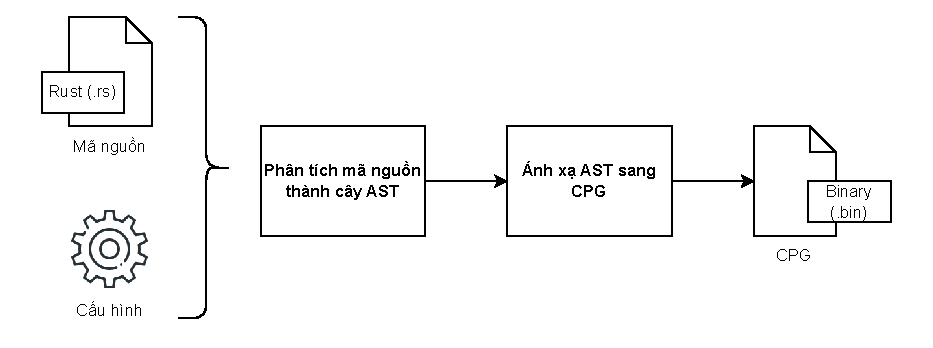
\includegraphics[width=1\columnwidth]{figures/c3/c3_flow.drawio.pdf}
	\centering
	\caption{Quy trình phân tích mã nguồn Rust.}
	\label{img:c3_flow}
\end{figure}

Mã nguồn Rust sẽ được trình phân tích và sinh ra cây AST tương ứng với từng tệp mã nguồn.
Sau đó, cây cú pháp trừu tượng sẽ được ánh xạ sang đồ thị thuộc tính mã nguồn.
Cuối dùng, đồ thị CPG sẽ được lưu dưới dạng cơ sở dữ liệu đồ thị phục vụ mục đích của người dùng.